%% Mapping (chpt5)
\chapter{Mapping} %10
The task of mapping was the main challenge of this work. This task consists in determining the 3D coordinates of recognizable features, that can later be used as landmarks by the drone to estimate its own position. The main challenge when building a 3D map using a single monocular camera, is that a point needs to be observed from at least 2 different positions to be mapped. The simplest approach to map a point, is to simply triangulate its position from two different views. We will begin by exploring this approach. We will find that although this does work reasonably well when we are certain of the position of the cameras, it does not when this position is uncertain. In addition, this method does not allow to take more than two observations of any point into account.\\

To remedy these problems we will implement a bundle adjustment step, that allows to build a map that is globally consistent. Throughout this section, we will have to make design choices to try to obtain a method that is both fast enough to work in real time, and accurate enough for the drone to control its position.\\

Finally we will implement a mapping strategy, that decides when and how to grow or reduce the map, and how to initialize it.

\section{Structure of the map}
We will keep the keyframe-based structure for the map from the previous years, but this structure will need to be adapted so that each landmark does not belong to just one keyframe. The map will contain two main data structures: a list of keyframes, and a list of landmarks. Each keyframe will contain the following information: the drone's pose estimation at the moment the keyframe was created, the estimated corrected pose of the keyframe, a list of observed keypoints. For each observed keypoint of this list, we also save its descriptor, its 2D position in the image plane of the keyframe, and whether it corresponds to a landmark of the map, and which one. Each landmark will contain a descriptor, its estimated 3D coordinates, and a list of keyframes seeing it. The map can be seen as a bipartite graph, where the landmarks and the keyframes form the two sets of nodes, and where an edge is present between a landmark and a keyframe if the keyframe sees the landmark.\\

The map grows every time we decide to add a keyframe. When we do, the keypoints of the current image seen by the camera, along with their 2D coordinates and descriptors, are saved in a new keyframe. The descriptors are then matched with descriptors of the other keyframes, and when there is a match between two keypoints of two different keyframes, we can triangulate a new landmark into the map.\\

\section{Triangulation} \label{sec:triangulation}
Our first problem is where to put a landmark in the 3D world from two observations at two different keyframes. If all measurements were perfect, we could simply draw a ray at each keyframe that goes from the camera center and passes through the keypoint in the image plane, and those two rays would intersect at the position of the landmark. \\

Unfortunately, those lines never intersect in practice, due to various errors (measurement errors, errors in the model of the cameras, errors on the position estimation of the cameras), so we need to find a method to locate a 3D point as best as possible from the pair of images.

\begin{figure}[H]
\centering
\begin{subfigure}{.5\textwidth}
  \centering
  \includegraphics[width=\linewidth]{triang_midpoint.png}
  \caption{Midpoint method}
  \label{fig:midpoint}
\end{subfigure}%
\begin{subfigure}{.5\textwidth}
  \centering
  \includegraphics[width=\linewidth]{triang_optimal.png}
  \caption{Optimal Correction}
  \label{fig:optimalcorrection}
\end{subfigure}%

\caption{Triangulation methods}
\label{fig:triang}
\end{figure}

\subsection{Midpoint Method}
The simplest and most obvious solution is to take the midpoint of the common perpendicular of the two rays. This method is intuitive to understand geometrically, and is quite easy to compute. In practice, however its results are not very good, as there is no theoretical reason for this point to be the best.

\subsection{Optimal Correction}
If we assume that the error on observed points is random and follows a Gaussian distribution with zero mean, then the optimal solution would be to displace the pixels on both images until the resulting rays meet, keeping the displacement of the pixels as small as possible in the least squared sense. Such a solution would give the maximum likelihood estimator of the position of the 3D point, under those assumptions.\\

There are several algorithms in the literature that triangulate the position of a point using optimal correction. The most popular one, proposed by Hartley and Sturm \cite{hartleysturm}, computes the solution directly but requires finding the root of a 6th degree polynomial. Kanantani et. al.'s method \cite{kanatani} finds a solution iteratively, but requires very few iterations to have an accurate solution, and in practice, is faster than the Hartley Sturm method. It also has better numerical properties, as unlike the Hartley-Sturm method, it does not have singularities at the epipoles.\\

As we will see in the results section (\ref{sec:comparetriang}), optimal correction performs better than the midpoint method, as could be expected. The performance increase from optimal correction is not very big however, because the biggest source of error is not Gaussian noise on the measurements of the points, but errors in the position estimate of the cameras at the moment of creating the keyframes.

\subsection{Angle between the rays}
It is interesting (and will be useful) to note that the accuracy of the triangulation depends on the angle between the two rays reaching the point. In the most extreme case, one of the two points from which the landmark is seen is exactly between the landmark and the other point, like on figure \ref{fig:anglesa}. Then the rays are parallel, the angle between them is \SI{0}{\degree} and the distance to the landmarks can't be determined. The same applies if the landmark is between the two points of view, and the angle is \SI{180}{\degree}, like on figure \ref{fig:anglesb}. The optimal situation lies between these two extreme cases, when the two rays form an angle of \SI{90}{\degree} like on figure \ref{fig:anglesc}. In practice, however, our scene is sufficiently far away so that this angle is always lower than \SI{90}{\degree}, so the larger the angle, the better.
\begin{figure}[H]
\centering
\begin{subfigure}{.28\textwidth}
  \centering
  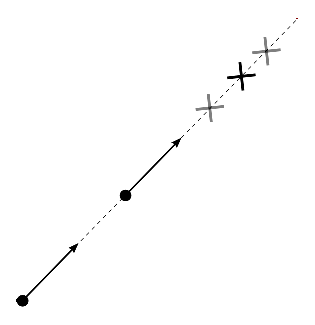
\includegraphics[width=\linewidth]{anglesa.eps}
  \caption{}
  \label{fig:anglesa}
\end{subfigure}%
\begin{subfigure}{.28\textwidth}
  \centering
  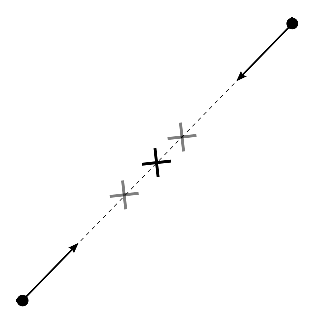
\includegraphics[width=\linewidth]{anglesb.eps}
  \caption{}
  \label{fig:anglesb}
\end{subfigure}%
\begin{subfigure}{.28\textwidth}
  \centering
  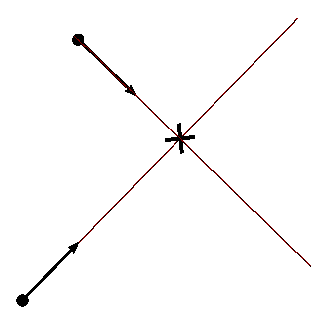
\includegraphics[width=\linewidth]{anglesc.eps}
  \caption{}
  \label{fig:anglesc}
\end{subfigure}%
\caption{Effect of the angle between the rays}
\label{fig:angles}
\end{figure}

\section{Bundle Adjustment}\label{sec:bundleadjustment}
Having a bad estimation of the keyframe's pose is problematic, as it will result in badly located landmarks, which in turn will cause a bad estimation of the camera's position when future keyframes are created. In the long term, errors will accumulate, and the map will be completely distorted. Luckily, if we have enough point correspondences between two images, it is possible to deduce the relative displacement between the two images. This means that from a set of images, we can reconstruct a scene, without even needing a prior estimation of the position of the cameras that took the images. This is good news as it means that the images can give us some absolute information about the scene, that can be used to correct the errors on the camera poses of the previous keyframes.\\

The problem of adjusting camera poses and 3D point locations in order to minimize the reprojection errors of the 3D points onto the image planes is known as bundle adjustment. Because bundle adjustment uses new information to correct older parts of the map, it allows to reduce the accumulation of errors. Another advantage of bundle adjustment, is that it can easily take into account points that are seen by more than two cameras, which is not trivial for the triangulation techniques described above. The main disadvantage of bundle adjustment is that it is computationally heavy, so it is important to adapt it to make it useable in real time.\\

Bundle Adjustment an optimization problem of a nonlinear least-squares problem. The problem can be described as follows:

\subsection{Variables and constants}
We are simultaneously trying to determine the layout of the drone's surroundings (landmarks) and to correct the estimations of the drone's poses at the previous keyframe locations. The variables we are optimizing are the previous keyframe poses and the 3D locations of the landmarks. Let $\mathcal{K}$ be the set of keyframes, $\mathcal{L}$ be the set of landmarks and $\mathcal{L}_k$ be the set of landmarks observed by keyframe $k$. We will call the camera centers of the previous keyframes $\mathbf{c}_k$ and their roll-pitch-yaw orientation angles $\mathbf{r}_k$. The 3D position of the landmarks will be called $\mathbf{p}_l$. For each observation of a landmark by a keyframe, we know at what 2D point on he image that point was observed. Let $\mathbf{i}_{lk}$ be the image coordinates of landmark $l$ in keyframe $k$.

\begin{table}[H] \caption{Table of notation for Bundle Adjustment}
  \centering
  \begin{tabular}{r c p{10cm} }
  \toprule
  \multicolumn{3}{c}{}\\
  \multicolumn{3}{c}{\underline{Constants}}\\
  \multicolumn{3}{c}{}\\
  $\mathcal{K}$   & $\triangleq$ & Set of keyframes\\
  $\mathcal{L}$   & $\triangleq$ & Set of landmarks\\
  $\mathcal{L}_k$ & $\triangleq$ & Set of landmarks seen by keyframe $k$\\
  $\mathbf{i}_{lk}$        & $\triangleq$ & Image coordinates of landmark $l$ in keyframe $k$'s image plane\\
  \multicolumn{3}{c}{}\\
  \multicolumn{3}{c}{\underline{Decision Variables}}\\
  \multicolumn{3}{c}{}\\
  $\mathbf{c}_k$           & $\triangleq$ & Position of camera center of keyframe $k$\\
  $\mathbf{r}_k$           & $\triangleq$ & Roll-pitch-yaw angles of camera of keyframe $k$\\
  $\mathbf{p}_l$           & $\triangleq$ & Position of landmark $l$\\
  \bottomrule
  \end{tabular}
  \label{tab:banotation}
\end{table}

$\mathrm{Proj}(\mathbf{p},\mathbf{c},\mathbf{r})$ is the projection operator. it transforms the 3D point coordinates $\mathbf{p}$ of any point into the 2D image coordinates of that point if it were perfectly observed by a keyframe located at position $\mathbf{c}$ with orientation $\mathbf{r}$. In addition of depending on the extrinsic camera parameters, ($\mathbf{c}$, and $\mathbf{r}$), this operator depends on the intrinsic (focal length, projection center, skew) parameters of the camera. In general, bundle adjustment refers to the problem of adjusting both the intrinsic and extrinsic camera parameters of the different keyframes, but in our case, the same camera is used at every location, and the intrinsic parameters have been found in advance using camera calibration. Therefore, we can simplify our model by taking the intrinsic parameters as known constants, and only solving for the extrinsic parameters and the position of the landmarks.

\subsection{Objective function} \label{sec:loss}
We want to minimize the reprojection error of the observed landmarks. After estimating $\mathbf{p}_l$, the position of landmark $l$, we can re-project point $l$ into the images it was observed from. For example, $\mathrm{Proj}(\mathbf{p}_l,\mathbf{c}_k,\mathbf{r}_k)$ is the reprojection of point $l$ into the image plane of camera $k$. We can then compare the reprojection with the actual observation of point $l$ by camera $k$ to find out how consistent the estimation of the position of point $l$ is with the estimation of the position and orientation of keyframe $k$. The objective then becomes:
\begin{equation} \label{eq:objfunc}
  \min \sum_{k\in\mathcal{K}}\sum_{l\in\mathcal{L}_k} L(\mathrm{Proj}(\mathbf{p}_l,\mathbf{c}_k,\mathbf{r}_k) - \mathbf{i}_{lk})
\end{equation}
for some loss function $L(\cdot)$. We would like to use a squared loss function, as it has good computational properties, but it has the disadvantage of giving a lot of weight to outliers. If some landmarks result from bad point correspondences, their reprojection errors will be very large, so they will influence the end result quite a lot. To reduce the effect of outliers, we use a more robust loss function: the Huber loss function.
\begin{equation} \label{eq:huber}
  L_\delta(x) = \left\{ \begin{array}{l l}
    \frac{1}{2} x^2 & \mathrm{if } |x| \leq \delta \\
    \delta|x| - \frac{1}{2}\delta^2 & \mathrm{otherwise} \end{array} \right.
\end{equation}
This function is equal to squared loss for values of $x$ smaller than $\delta$, and becomes straight line elsewhere. \\

Note that if we kept the keyframe positions and orientations constant, and if there were only 2 keyframes observing each landmark, then the triangulation obtained with optimal correction would already give us the landmark positions that minimize this reprojection error. The interest of using bundle adjustment is that it allows to correct the positions of the camera at the keyframes, and to consider more than two observations per landmark.

\subsection{Constraints}
Bundle Adjustment is generally an unconstrained problem, but we will add some soft constraints to incorporate information we have from the sensors. We will add terms to the objective function that penalize keyframes whose altitude, roll, and pitch are far away from the ones measured during the keyframe creation. Because each of these measures is absolute, they are not subject to drift, so they should be accurate even after the drone travels large distances. Doing this will prevent the solution of the bundle adjustment taking unrealistic values. \\

Another advantage is that this will (softly) fix the scale. As we said before, monocular vision only gives information of the world up to a scale factor, and bundle adjustment is normally unable to recover the real scale of the map it builds. Enforcing a constraint on the altitude of the keyframes fixes this scale, on the condition that the altitudes of the different keyframes vary, because then it gives a constraint on the distance between keyframes. For this reason, making the second keyframe from a position directly above the first one is a good idea.


\subsection{Solver}
We have a least square problem of the form:
\begin{equation} \label{eq:solver}
  \min_{x} G(x) = ||F(x)||^2
\end{equation}
Where $F$ is a highly non-linear, non-convex function as defined in \ref{eq:objfunc}. Because F is non-linear and non-convex, we can only hope to minimize it locally, using an iterative algorithm, so it will be very important to start from initial solutions that are close to the optimum. At each iteration, we want to find a step $\Delta x$ that brings the objective $F(x+\Delta x)$ closer to zero. We use the first-order approximation of $F(x + \Delta x)\approx F(x) + J(x)\Delta x$, where $J(x) = \left[\frac{\partial F_i}{\partial x_j}\right]$ is the Jacobian of $F$. Deriving \ref{eq:solver} with respect to $\Delta x$ with this approximation and setting it to zero gives the Gauss-Newton update:
\begin{equation}\label{eq:gaussnewt}
	\left( J^TJ\right)\Delta x = -J^TF
\end{equation}
By adding a regularization term $\lambda I$ to equation \ref{eq:gaussnewt}, we obtain Levenberg's update:
\begin{equation}
	\left( J^TJ + \lambda I \right)\Delta x = -J^TF
\end{equation}
Marquardt later improved this update by replacing $\lambda I$ by $\lambda\texttt{diag}(J^TJ)$, for faster convergence when $\lambda$ is large.\\

When the value of $\lambda$ is very small, the Levenberg-Marquardt update is quite close to a Gauss-Newton update, and when it is large, it becomes close to a gradient update. The Levenberg-Marquardt algorithm can be seen as a hybrid between the two. After each iteration, $\lambda$ is increased if we are getting closer to a minimum, or decreased if the iteration results in a worse value of the objective function. As a result, when the $2^{nd}$ order approximation is good, the method is close to a Gauss-Newton method, and very fast, and when it is bad, the method reverts to a gradient descent for stability.\\

To measure how good the approximation is we use $\rho$, a metric to compare the gain in the objective function with the one we would have gotten if the approximation was exact:
\begin{equation}\label{eq:metric}
	\rho = \frac{G(x) - G(x + \Delta x)}{G(x) - ||(F(x) + J(x)\Delta x)||^2}
\end{equation}
After each iteration, if $\rho$ is above some threshold, we perform the step : $x_{\texttt{new}} =x + \Delta x$ and $\lambda$ is decreased by some factor, if not, we do not update the value of $x$, and $\lambda$ is increased. We stop the algorithm when either the gradient, or the relative update of the parameters ($|\frac{\Delta x}{x}$) falls below some threshold. \cite{levmar}


\section{Mapping Strategy}\label{sec:mapstrat}
The last remaining task of the mapping task is to put all these elements together to build the mapping algorithm. This algorithm needs to decide how to initialize the map, when to create new keyframes, when and how to run bundle adjustment, and how to limit the growth of the map.

\subsection{Map Initialization}
Because of the chicken-and-egg nature of SLAM (an estimate of the position is necessary to place landmarks, but a map is necessary to estimate the position), a special procedure is needed to initialize the map. Arbitrarily, we decide to place the origin of our reference frame at the pose of the drone where it creates the first keyframe, with the x direction pointing forwards, the y direction to the left, and the z direction upwards (this is the coordinate system used by \texttt{ardrone\_autonomy}). The first keyframe will serve as the anchor of the map: its position will never change, and will always stay at the origin.\\

A single keyframe is not enough to initialize a map, because two views of keypoints are required to triangulate them. This means we have to fly blindly to the location of the second keyframe before we can create any landmarks, and begin to estimate the drone's position using the map and PnP. The only available sensors during this first, blind flight are the IMU, the ultrasonic sensor, and the bottom camera (for optical flow). Of these, only the ultrasonic sensor gives an absolute measurement of position, the others all measure speed, and this speed estimation has to be integrated to give a displacement estimate. For this reason, we will mostly rely on the ultrasonic sensor to estimate the relative displacement between the two first keyframes. Because the ultrasonic sensor only gives the distance from the bottom of the drone to the ground, the drone should fly straight up from its first position (the origin) to reach its second position.\\

Once in its second position, the drone can match seen keypoints from both views, and from its estimated position, triangulate those points to the map. Then, using bundle adjustment, the error in the estimation of the displacement between the two first keyframes can be corrected.

\subsection{Local and global bundle adjustment}\label{sec:locglob}
As we will see in chapter \ref{chpt:results}, the time taken for bundle adjustment will be one of the major obstacles of this work. This time taken depends on the number of points and keyframes concerned, so as the map grows, it will become impractical to run bundle adjustment on all of it. For this reason, we will only solve bundle adjustment on a subset of the map, considering only the most recent keyframes, and the points seen by them. This will allow to put a cap on the size of the problem that has to be solved each time a keyframe is created. Confining bundle adjustment to a local window means that errors will still accumulate over time, but still much more slowly than with no bundle adjustment. To solve this, we can occasionally run bundle adjustment on the whole map, which would be especially useful if the drone revisits a previously seen location.

\subsubsection{Local Bundle Adjustment}
Every time a keyframe is created, we follow this creation with a round of local bundle adjustment, to correct the error due to the inaccuracy of this keyframe's position. When running local bundle adjustment, we only solve a sub-problem of the full bundle adjustment. In this sub-problem, we only consider the $n$ last keyframes, and the landmarks seen by at least two of those $n$ keyframes.\\

We will set the poses of the two oldest keyframes considered in the local bundle adjustment as constant. This is necessary to prevent drift. It there was no keyframe set as constant, the entire map could be shifted with no effect on the objective function. Likewise, if there was only one keyframe set as constant, the entire map could be scaled by a factor around the constant keyframe, with no change to the objective function. The two constant keyframes serve as anchor of the local map, fixing its position within the global map. Choosing the oldest keyframes to be set as constant ensures that the constant keyframes have already been through some ($n - 2$) rounds of local bundle adjustment, so we can expect their position to already be close to the correct one, or at least to be locally consistent with the map.

\subsubsection{Global Bundle Adjustment}
As local bundle adjustment only considers a sub-problem, its solution is not optimal with respect to the full problem. When the drone has processor time available, we can improve our solution by running the algorithm on the full problem. When doing this, we are modifying all keyframes except for the first one, the anchor of the global map. The keyframes that are normally kept constant during local bundle adjustment are also modified, correcting some of the accumulated error that was made until there. However, errors will still accumulate as the drone moves away from the global anchor. These accumulated errors can be corrected if there are loops in the drone's trajectory, but they do not prevent the drone from exploring because the map stays locally consistent.


\subsubsection{Loop Closure}
Each landmark couples the positions of all keyframes seeing them: modifying the position of one keyframe changes the optimal position of the landmark, which changes the optimal position of the other keyframes. We can consider keyframes to be neighbors if they see a common landmark. Having keyframes that are far away from each other, in the sense that many intermediate keyframes are required to go from one to the other, traveling from neighbor to neighbor, means that the two keyframes are very loosely coupled. The looser keyframes are coupled from the first keyframe, the more they are subject to drift, as the errors accumulate between them.\\

Using local bundle adjustment further increases this drift, as keyframes whose positions are not simultaneously optimized during bundle adjustment are only coupled through the anchors of the local bundle adjustment, not directly though point correspondences. When running global bundle adjustment, this drift can be corrected, especially when the keyframes are strongly coupled. The best situation for this is when the drone makes a full loop, and revisits locations seen by much older keyframes. The newest keyframes then become neighbors to the oldest, and global bundle adjustment can correct all the errors accumulated during the loop, resulting in a completely consistent map.

\subsection{Rejecting outliers}
When looking more closely at the results of bundle adjustment, we find that despite the use of a robust loss function (see section \ref{sec:loss}) a large part of the errors comes from a small number of points. Figure \ref{fig:errorrepartition} shows the repartition of contribution to the objective function between the landmarks (a logarithmic scale is used for the $x$-axis). We can see that \SI{1}{\percent} of the landmarks account for more than \SI{40}{\percent} of the total error, and that \SI{10}{\percent} of the landmarks account for more than \SI{80}{\percent} of the total error.  One possible explanation is that these points are bad matches, and do not correspond to real world points, so that even if we have the correct position of all cameras exactly, the rays corresponding to these points will not intersect.

\begin{figure}[H]
  \centering
  \includegraphics[scale=0.6]{err_repartition_4.eps}
  \caption{Repartition of error among points}
  \label{fig:errorrepartition}
\end{figure}

To solve this problem, after every bundle adjustment pass, we eliminate points whose error is higher than some threshold to be defined. Because the number of keyframes seeing each individual landmark varies, we should look at the error per observation of each point. It is also normal that the error per observation becomes larger for points observed by more keyframes, because every time an observation is added, the location of the point will change a bit, and its position will become less optimal with respect to the keyframes that already saw it.\\

For these reasons, we will put a different threshold on the points depending on the number of keyframes that see the point. If a point is seen by a large number of keyframes, we will allow it to have larger errors per observation before removing it.\\

As we will see in \ref{sec:outliers}, removing outliers greatly improves the performance.


\subsection{Choosing when to create keyframes}\label{sec:heuristic}
Choosing when to create keyframes was the most challenging task of this work. It is not a simple tradeoff between computation time and accuracy, as many (sometimes contradicting) points have to be kept in mind:
\begin{itemize}
\item Landmarks have to be observed from at least two keyframes before they can be used, so it is important to create keyframes sufficiently in advance
\item If two keyframes are too close to one another, the lines going from landmarks to these two keyframes will almost be parallel, causing a large uncertainty on the landmark's position
\item It is important to have a good pose estimate at the moment a keyframe is created, as this estimate will be the initial value of the keyframe's pose
\item Because when we add a keyframe we run a local bundle adjustment on the last $n$ keyframes, if the keyframes come in rapid succession, errors will accumulate faster, as there are more intermediates between the first and last keyframes.
\end{itemize}

The choice of when to create a new keyframe has to be made heuristically using any of the measures we have available. Amongst the quantities considered for this choice are:
\begin{itemize}
\item The time elapsed since the last keyframe was created
\item The distance to the position where the last keyframe was created
\item The distance to the position of other keyframes
\item The number of mapped points currently in the field of view
\item The number of unmapped points currently in the field of view
\item The number of inliers the last times RANSAC was run
\item Large areas in the field of view not containing any mapped points
\end{itemize}

After many trial-and-error tests, we came up with the following heuristic:

\begin{itemize}
\item{If bundle adjustment is currently running, don't create a keyframe}
\item{If the current position (disregarding orientation) is closer than \SI{10}{\centi\meter} to the last keyframe, don't create a new keyframe}
\item{The is no area larger than \SI{20}{\percent} of the image on any of the 4 sides that contains no RANSAC inliers}
\item{If any of the following conditions is true, create a new keyframe:}
\begin{itemize}
	\item{The current position (disregarding orientation) is farther than \SI{70}{\centi\meter} from the last keyframe}
	\item{An area larger than \SI{33}{\percent} of the image (from any of the 4 sides) contains no RANSAC inliers}
	\item{The current image contains less than 40 RANSAC inliers}
\end{itemize}
\end{itemize}

The reason we use the distance between poses, disregarding orientation, is that if one keyframe results from the drone performing a pure rotation from another keyframe, the rays between points of the scene and the keyframes will be close to parallel in the reference coordinate system, and cause resulting landmarks to have a large uncertainty. For this reason, it is also important that the path-planning node (not worked on in this thesis) avoids pure rotations.

\section{Summary}
Every time the mapping node receives a new frame from the computer vision node, it decides whether a new keyframe is needed, using the heuristic described in section \ref{sec:heuristic}. If a new keyframe is needed, the frame is transformed into a keyframe, the list of keypoints, each with their descriptor and 2D position on the image is saved, and the estimated position of the drone at the moment of creating the keyframe is assigned to the keyframe. The descriptors of the new keyframe are then matched with the descriptors of already mapped landmarks and with the descriptors of currently unmatched keypoints in older keyframes. If there is a match between two unmatched keypoints in different keyframes, a new landmark is created by triangulating its position with optimal correction (see section \ref{sec:triangulation}).\\

For each keypoint in each keyframe, we also save whether it corresponds to any landmark of the map. After the keyframe is created, we decide whether to run local or global bundle adjustment, as explained in section  \ref{sec:locglob}. We then run bundle adjustment (section \ref{sec:bundleadjustment}), either on the entire map if we decided to run global bundle adjustment, or on the last $n$ keyframes and the landmarks seen by at least two of those if we decided to run local bundle adjustment. Running bundle adjustment allows to use the matches between keypoints to correct the estimations of the positions of those keypoints and the keyframes seeing them.\\

Figure \ref{fig:mapflowchart} summarizes the mapping part of the code in the form of a flowchart. Bundle adjustment runs in a separate node, so that it doesn't block the entire mapping node.

\begin{figure}[H]
  \centering
  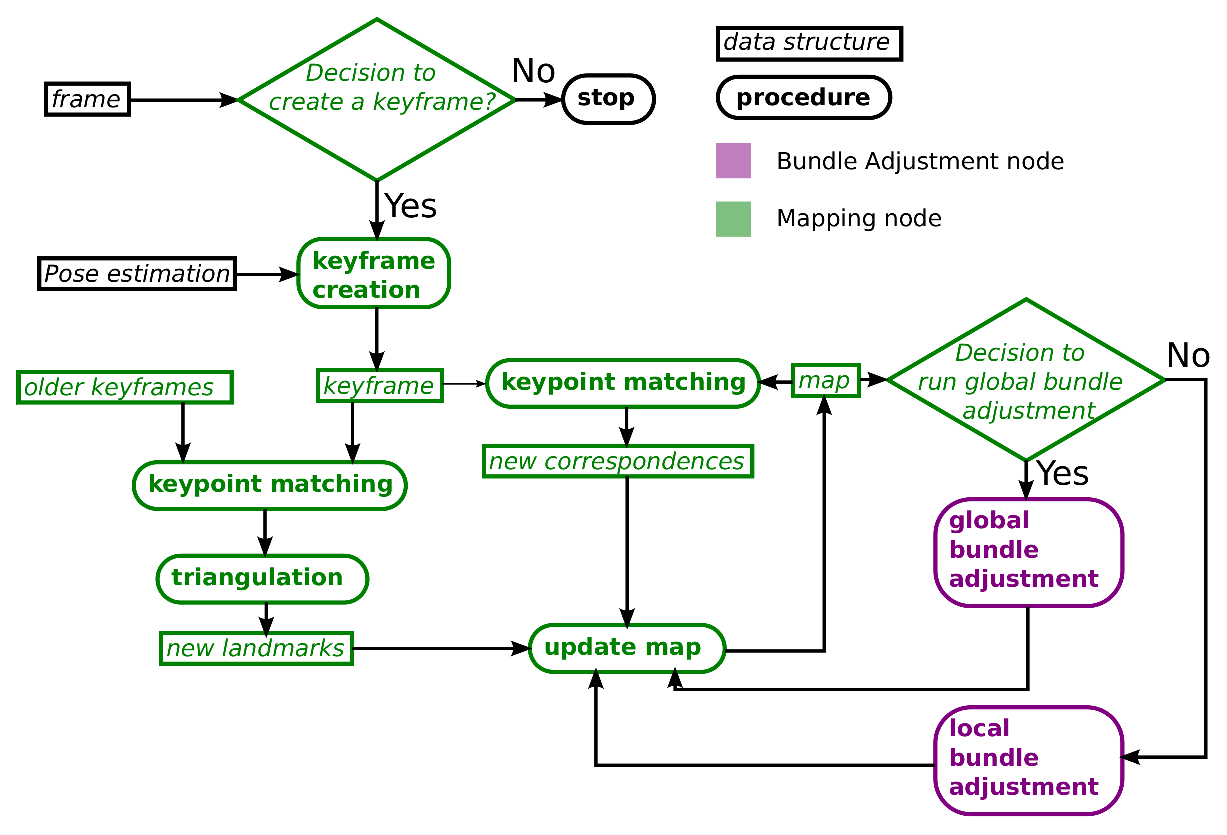
\includegraphics[scale=0.6]{mapflowchart.eps}
  \caption{Flowchart of the mapping task}
  \label{fig:mapflowchart}
\end{figure}
